\part{The Lifecycle at a Glance}

\chapter{The whole project on a few pages}
\label{r:ch:overview}

\section{The question}

Public cervical cytology benchmarks are released as cell crops, and most crops are cut from far fewer microscope
fields or slide images. When a benchmark is split at the crop level, crops from one field land on both sides of the
train--test boundary. Files are disjoint, but the test set shares stain, illumination, focus, background, and sometimes
literal pixels with training. The project asked three questions in order: \emph{is the structure there}, \emph{is the
shared parent recognisable}, and \emph{does it inflate reported performance}; and then a fourth: \emph{how do models use
it}.

\section{What happened, in order}

\begin{figure}[H]
\centering
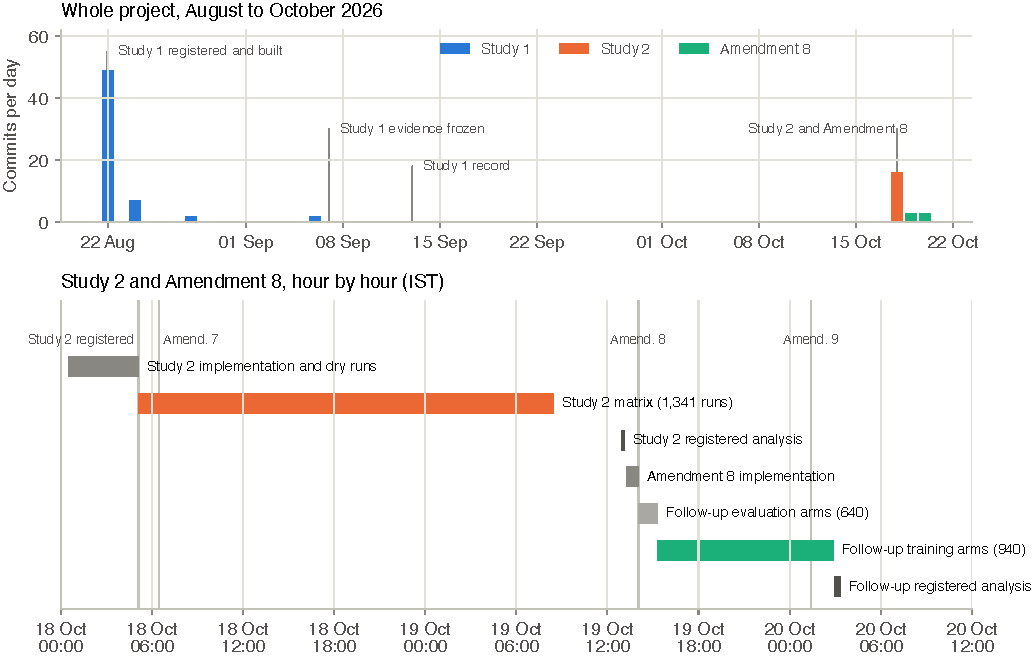
\includegraphics[width=\textwidth]{timeline.pdf}
\caption{The lifecycle. Top: commits per day across the project. Bottom: Study~2 and Amendment~8 hour by hour; every
span is measured from run records or commits.}
\label{r:fig:timeline}
\end{figure}

\begin{figure}[H]
\centering
\begin{adjustbox}{max width=\textwidth}
\begin{tikzpicture}[node distance=5mm and 6mm]
\node[done=30mm] (s1reg) {Study 1 registered\\\footnotesize 22 Aug 2026};
\node[done=30mm, right=of s1reg] (s1run) {Provenance, structure,\\probe, 325 models};
\node[gold=30mm, right=of s1run] (s1res) {Inflation not certified\\\footnotesize 6 tests, none survive BH};
\node[box=30mm, below=of s1res] (rec) {Study 1 record\\\footnotesize frozen 7--13 Sep};
\node[box=30mm, left=of rec] (road) {Scaling roadmap\\\footnotesize review of weaknesses};
\node[box=30mm, left=of road] (p0) {Phase 0 checks\\\footnotesize clone, licence, Cx22 lit.};
\node[done=30mm, below=of p0] (s2reg) {Study 2 registered\\\footnotesize 18 Oct 05:07};
\node[gold=30mm, right=of s2reg] (a7) {Amendment 7\\\footnotesize failure handling};
\node[done=30mm, right=of a7] (s2run) {1,341 runs\\\footnotesize 27 h on 4 GPUs};
\node[done=30mm, below=of s2run] (s2res) {H1, H2, H3 supported\\H4, H5 not};
\node[done=30mm, left=of s2res] (a8) {Amendment 8 registered\\\footnotesize 19 Oct 14:02};
\node[done=30mm, left=of a8] (frun) {1,580 follow-up tasks\\\footnotesize 13 h on 4 GPUs};
\node[bad=30mm, below=of frun] (a9) {Amendment 9\\\footnotesize preparer bug, no output};
\node[done=30mm, right=of a9] (fres) {F2, F3 supported\\F1, F4--F8 not};
\node[box=30mm, right=of fres] (paper) {Manuscript, record,\\archive, vacate};
\draw[flow] (s1reg) -- (s1run); \draw[flow] (s1run) -- (s1res); \draw[flow] (s1res) -- (rec);
\draw[flow] (rec) -- (road); \draw[flow] (road) -- (p0); \draw[flow] (p0) -- (s2reg);
\draw[flow] (s2reg) -- (a7); \draw[flow] (a7) -- (s2run); \draw[flow] (s2run) -- (s2res);
\draw[flow] (s2res) -- (a8); \draw[flow] (a8) -- (frun); \draw[flow] (frun) -- (a9);
\draw[flow] (a9) -- (fres); \draw[flow] (fres) -- (paper);
\end{tikzpicture}
\end{adjustbox}
\caption{The whole lifecycle as a sequence of registered decisions (green), amendments and setbacks (gold, red),
and reviews (blue). Every arrow is a commit in the repository; Appendix~\ref{r:app:git} lists all of them.}
\label{r:fig:lifecycle-flow}
\end{figure}


\begin{enumerate}[leftmargin=1.8em]
\item \textbf{Study 1 (22 August -- 13 September 2026).} The crop-to-parent hierarchy of four public datasets was
recovered with independent, fail-closed branches; random crop splitting placed a training parent behind 92.6\% of
SIPaKMeD and 99.97\% of CRIC test cells; more than half of SIPaKMeD test crops shared source pixels with a training
crop; a 424-way parent probe reached 109 times chance. Classifiers scored higher under crop-level splits for all six
architectures and all seven Cx22 segmentation models, but none of the per-architecture tests survived the registered
Benjamini--Hochberg correction. Part~II is that record.
\item \textbf{The roadmap (October 2026).} A review identified four weaknesses: one question asked six times, availability
not distinguished from use, leakage confounded with training diversity, and only one rescored benchmark. It proposed a
single mixed-model test sized by simulation, causal arms, more architectures and seeds, preregistration, and keeping
every per-sample artifact (Chapter~\ref{r:ch:roadmap}).
\item \textbf{Study 2 (18--19 October).} Registered at commit \texttt{\RegistrationCommit} (\RegistrationTime), before any
Study~2 model was trained: one primary test (H1) and a Holm family of four mechanism tests (H2--H5), \RecStudyTwoRuns\
runs over \RecStudyTwoWall\ hours on four GPUs. H1, H2, and H3 were supported; H4 and H5 were not.
\item \textbf{Amendment 8 (19--20 October).} Eight new hypotheses about \emph{how} the leak is used, registered at
\texttt{\FollowupCommit} (\FollowupTime) after the Study~2 analysis and before any follow-up run: \RecFollowTasks\ tasks
over \RecFollowWall\ hours. F2 and F3 were supported; F1 went the opposite way; F4--F8 were null.
\item \textbf{Amendment 9 (20 October, 01:25).} A labelling bug in the follow-up preparer halted the analysis before it
produced output; fixed and recorded before any affected estimate was seen.
\item \textbf{Close-out.} Manuscript (\artifact{paper/v2}), this record, 121~GB of outputs archived and verified on the
network home, and the node-local disk vacated.
\end{enumerate}

\section{Every registered test}

{\footnotesize
\setlength{\tabcolsep}{3.5pt}
\begin{longtable}{llrrrrl}
\caption{Every registered confirmatory test of Study 2 and Amendment 8. H1 is tested alone; H2--H5 and F1--F8 are separate Holm families. Units as in the text (pp; slopes in pp per pp).}\label{r:tab:alltests}\\
\toprule
 & Question & Estimate & 95\% CI & $p$ & Holm $p$ & Verdict \\
\midrule
\endfirsthead
\toprule
 & Question & Estimate & 95\% CI & $p$ & Holm $p$ & Verdict \\
\midrule
\endhead
\bottomrule
\endfoot
H1 & SIPaKMeD P1 $-$ P2 accuracy (primary) & 0.97 & 0.59 to 1.39 & $<$0.001 & alone & \supported \\
H2 & CRIC P1 $-$ P2 accuracy & 12.08 & 11.16 to 12.99 & $<$0.001 & $<$0.001 & \supported \\
H3 & 2C leakage at matched diversity & 1.73 & 0.95 to 2.51 & 0.006 & 0.02 & \supported \\
H4 & 2B own-context route & 0.42 & \textminus{}0.35 to 1.18 & 0.23 & 0.23 & \notsupported \\
H5 & 2A gap vs recoverability & 0.059 & \textminus{}0.007 to 0.125 & 0.08 & 0.16 & \notsupported \\
F1 & CRIC slide-context pull & \textminus{}4.29 & \textminus{}8.60 to \textminus{}1.37 & $<$0.001 & 0.001 & \notsupported \\
F2 & test-time stain transfer & 1.27 & 0.38 to 2.16 & 0.005 & 0.03 & \supported \\
F3 & leak with backgrounds masked & 1.86 & 1.42 to 2.30 & $<$0.001 & $<$0.001 & \supported \\
F4 & colour augmentation & \textminus{}0.23 & \textminus{}0.81 to 0.35 & 0.43 & 1.00 & \notsupported \\
F5 & LEACE erasure & \textminus{}0.01 & \textminus{}0.10 to 0.07 & 0.72 & 1.00 & \notsupported \\
F6 & stain normalisation & 0.02 & \textminus{}0.41 to 0.44 & 0.94 & 1.00 & \notsupported \\
F7 & probe-matched adversary & 0.000 & \textminus{}0.038 to 0.039 & 0.99 & 1.00 & \notsupported \\
F8 & pooled dose-response & 0.000 & \textminus{}0.005 to 0.005 & 0.93 & 1.00 & \notsupported \\
\end{longtable}
}


\begin{figure}[H]
\centering
\begin{adjustbox}{max width=\textwidth}
\begin{tikzpicture}[node distance=3mm and 5mm, every node/.style={font=\small}]
\node[box=34mm] (c1) {\textbf{Structural non-independence}\\test cells share a parent};
\node[box=34mm, below=8mm of c1] (c2) {\textbf{Shortcut availability}\\the parent is recognisable};
\node[box=34mm, below=8mm of c2] (c3) {\textbf{Consequence}\\scores are inflated};
\node[box=34mm, below=8mm of c3] (c4) {\textbf{Mechanism}\\how the leak is used};
\node[done=48mm, right=10mm of c1] (t1) {Study 1: 92.6\% (SIPaKMeD), 99.97\% (CRIC) test cells with a training parent; Herlev 0\%};
\node[done=48mm, right=10mm of c2] (t2) {Study 1: 424-way probe 109$\times$ chance; 79$\times$ with the cell inpainted away};
\node[done=48mm, right=10mm of c3] (t3) {Study 2: H1 +\HoneEst~pp, H2 +\HtwoEst~pp, H3 +\HthreeEst~pp (leakage, not diversity), replicated};
\node[gold=48mm, right=10mm of c4] (t4) {H4, H5 not supported; A8: F2, F3 supported, F1 reversed, F4--F8 null};
\node[note, right=4mm of t1, text width=26mm] {established};
\node[note, right=4mm of t2, text width=26mm] {established};
\node[note, right=4mm of t3, text width=26mm] {established};
\node[note, right=4mm of t4, text width=26mm] {narrowed by elimination};
\foreach \a/\b in {c1/t1,c2/t2,c3/t3,c4/t4} \draw[flow] (\a) -- (\b);
\draw[flow] (c1) -- (c2); \draw[flow] (c2) -- (c3); \draw[flow] (c3) -- (c4);
\end{tikzpicture}
\end{adjustbox}
\caption{The four claims the project separates, and the evidence each received. Study 1 established the first two;
Study 2 the third; Amendment 8 narrowed the fourth.}
\label{r:fig:hypothesis-map}
\end{figure}


\section{What we got out of it}

\begin{workedbox}{Established}
\begin{itemize}[leftmargin=1.4em]
\item Crop-level splitting inflates accuracy on SIPaKMeD by \HoneEst~pp (95\% CI \HoneBootLo--\HoneBootHi; all
twelve architectures positive) and on CRIC by \HtwoEst~pp; the parent-level error rate is \SipErrorRatio\ and
\CricErrorRatio\ times the crop-level one.
\item The inflation is leakage, not the extra training diversity crop-level splits bring: at matched crop and field
counts the leak effect is \HthreeEst~pp and the diversity effect \DivEst~pp; the leak effect replicated on fresh seeds
(\HthreeRepEst~pp).
\item The leak needs no background (F3: \FthreeEst~pp with every background masked) and is tied to the field's colour
rendering at test time (F2: stain transfer cuts it from \LeakUnderOriginal\ to \LeakUnderStain~pp).
\item Neither a linearly decodable field code nor Grad-CAM-visible attention carries it: erasing or adversarially
suppressing field identity cut probe recoverability by up to \RecoveryCutMax\% without moving the gap, and Grad-CAM maps
of leak and clean models were indistinguishable.
\end{itemize}
\end{workedbox}

\begin{warningbox}{Not supported, reversed, or open}
\begin{itemize}[leftmargin=1.4em]
\item H4 (a background context route) and H5 (the gap tracks gradient-reversal suppression) were not supported; the
ConvNeXt-T adversary was evaded.
\item F1 reversed: CRIC models were \emph{not} pulled toward the slide's majority label.
\item F4: strong colour augmentation did not prevent leakage, which qualifies F2.
\item Parents are not patients; one training recipe was used throughout; Study~2's registrations still need an external
timestamp.
\end{itemize}
\end{warningbox}

\begin{decisionbox}{The practical message}
Probes, saliency maps, background removal, and colour augmentation cannot certify that an evaluation is free of
hierarchical leakage. Only a split at the deepest released parent unit removes it, and the closed forms of
Chapter~\ref{r:ch:structure} predict which benchmarks are exposed before any model is trained.
\end{decisionbox}

\section{Numbers at a glance}

\begin{longtable}{p{0.55\textwidth}p{0.38\textwidth}}
\toprule
Quantity & Value \\
\midrule
Trained models (Study 1, Study 2, Amendment 8) & \RecAllModels\ (325 + \RecStudyTwoRuns\ + \RecFollowTrainRuns) \\
Evaluation-only runs on saved models (Amendment 8) & \RecFollowEvalRuns \\
Training epochs logged (Study 2 and Amendment 8) & \RecEpochs \\
GPU-hours, Study 2 / Amendment 8 & \RecGpuHoursStudyTwo\ / \RecGpuHoursFollow \\
Study 2 matrix wall clock & \RecStudyTwoWall\ h (\RecStudyTwoStart\ to \RecStudyTwoEnd) \\
Amendment 8 matrix wall clock & \RecFollowWall\ h (\RecFollowStart\ to \RecFollowEnd) \\
Failed tasks, retries, diverged runs & 0, 0, 0 \\
Smoke tests before registration & \RecSmokeRuns \\
Commits & \RecCommits \\
Registered confirmatory tests & 1 primary + 4 (Holm) + 8 (Holm) \\
\bottomrule
\end{longtable}
